\documentclass[11pt,aspectratio=169]{beamer}
\usetheme{CambridgeUS}
\usecolortheme{beaver}
\setbeamertemplate{navigation symbols}{}
\usepackage[utf8]{vietnam}
\usepackage{booktabs}
\usepackage{graphicx}
\usepackage{amsmath}
\usepackage{gensymb}
\usepackage{setspace}
\usepackage{pgfplots}
\onehalfspacing
\title{Chính sách thuế của chính phủ đến thị trường thuốc lá}
\author{Nhóm 15}
\date{November 2024}
\begin{document}
\maketitle
\begin{frame}{Mục lục}
\begin{itemize}
    \item Tổng quan
    \item Phương trình hàm cung và cầu
    \item Xác định điểm cân bằng $E$ của đồ thị
    \item Kết luận
\end{itemize}
\end{frame}
\begin{frame}{Tổng quan}
    \begin{itemize}
        \item Việt Nam là một trong những quốc gia có tỷ lệ người hút thuốc cao nhất thế giới với khoảng $41.1\%$ người hút thuộc đối tượng nam giới trưởng thành và có gần $20.8\%$ dân số hút thuốc.
        \item Thuốc lá là mặt hàng bị Chính phủ đánh thuế rất cao nhằm làm giảm số lượng người hút do các lo ngại với sức khỏe.
        \item Trong năm 2020, khi đại dịch COVID-19 bùng phát, mặt hàng thuốc lá đã bị áp \textbf{thuế tiêu thụ đặc biệt} với mức thuế gián tiếp lên tới $10$ nghìn đồng.
        \item Ta sẽ tập trung khảo sát tác động của mức thuế này lên mặt hàng thuốc lá với các đối tượng người tiêu dùng, nhà sản xuất và Chính phủ.
    \end{itemize}
\end{frame}
\begin{frame}{Phương trình hàm cung và cầu}
    \begin{center}
    \begin{tabular}{llrll}
        \toprule
        $P$   & $Q_{s}$   & $Q_{d}$  \\
        \midrule
         15    & 4.0   & 5.0  \\
         16    & 4.3   & 4.8  \\
         17    & 4.6   & 4.6  \\
         18    & 4.9   & 4.4 \\
         19    & 5.2   & 4.2 \\
         20    & 5.5   & 4.0 \\
        \bottomrule
        \end{tabular}
    \end{center}
(Đơn vị của $P$ là nghìn đồng, của $Q_{s}$ và $Q_{d}$ là triệu gói)
\end{frame}
\begin{frame}
Ta có phương trình tuyến tính tổng quát của hàm cung $Q_{s}$ và hàm cầu $Q_{d}$ với $a, b, c, d$ là các tham số tương ứng:
\begin{equation*}
    \begin{cases}
    Q_{s}=a+bP\\
    Q_{d}=c-dP\\
    \end{cases}
    \end{equation*}
Từ dữ kiện của bảng cung và cầu đã có ở trên, ta có thể dễ dàng xác định được phương trình của hàm cung $Q_{s}$ và hàm cầu $Q_{d}$ là:
\begin{equation*}
    \begin{cases}
    Q_{s}=-0.5+0.3P\\
    Q_{d}=8-0.2P\\
    \end{cases}
    \end{equation*}
Sau khi đã xác định được phương trình $Q_{s}$ và $Q_{d}$, ta có thể vẽ đồ thị như sau:
\end{frame}
\begin{frame}
    \begin{center}
    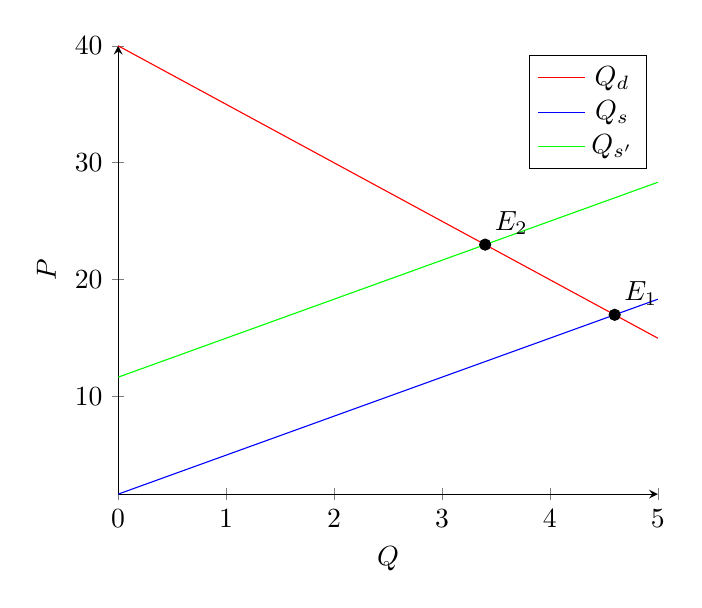
\begin{tikzpicture}
        \begin{axis}[
            axis lines = left,
            xlabel = \(Q\),
            ylabel = {\(P\)},
        ]
        %Below the red parabola is defined
        \addplot [
            domain=0:5, 
            samples=10, 
            color=red,
        ]
        {-5*x+40};
        \addlegendentry{\(Q_{d}\)}
        %Here the blue parabola is defined
        \addplot [
            domain=0:5, 
            samples=100, 
            color=blue,
            ]
            {x*3.3333+1.666666};
        \addlegendentry{\(Q_{s}\)}
        \addplot [
            domain=0:5, 
            samples=100, 
            color=green,
            ]
            {x*3.3333+11.666666};
        \addlegendentry{\(Q_{s'}\)}
        \addplot[mark=*] coordinates {(4.6,17)};
        \addplot[mark=*] coordinates {(3.4,23)};
        \node[anchor=south west] at (axis cs:4.6,17) {$E_{1}$};
        \node[anchor=south west] at (axis cs:3.4,23) {$E_{2}$};
        \end{axis}
        \end{tikzpicture}
    \end{center}
\end{frame}
\begin{frame}{Xác định điểm cân bằng $E$ của đồ thị}
\begin{enumerate}
    \item Khi mặt hàng thuốc lá chưa bị đánh thuế, ta thấy điểm cân bằng $E_{1}$ có tọa độ thỏa mãn phương trình:
$$Q_{s}=Q_{d} \Leftrightarrow -0.5+0.3P=8-0.2P$$
\begin{equation*}
    \Leftrightarrow
    \begin{cases}
    P=17\\
    Q=4.6\\
    \end{cases}
    \end{equation*}
    Vậy điểm cân bằng $E_{1}$ có tọa độ là $(4.6, 17)$.
    \item Khi mặt hàng thuốc lá bị Chính phủ đánh thuế gián tiếp $10$ nghìn đồng, ta dễ thấy đồ thị hàm $Q_{s}$ sẽ bị dịch lên trên một đoạn ở trục tung Price (do bị áp thuế) và trở
thành đường $Q_{s'}$ có phương trình: $Q_{s'}=-0.5+0.3(P-10)$.
\end{enumerate}
\end{frame}
\begin{frame}
Giải phương trình để tìm điểm cân bằng $E_{2}$, ta có:
$$Q_{s'}=Q_{d}\Leftrightarrow -0.5+0.3(P-10)=8-0.2P$$
\begin{equation*}
    \Leftrightarrow
    \begin{cases}
    P=23\\
    Q=3.4\\
    \end{cases}
    \end{equation*}
\end{frame}
\begin{frame}{Kết luận}
Vậy từ các số liệu đã tính được, ta có thể đưa ra các kết luận sau:
\begin{itemize}
    \item Sau khi bị áp thuế, giá bán lẻ của mỗi gói thuốc lá đã tăng lên $\Delta P=23-17=6$ (nghìn đồng) với người tiêu dùng.
    \item Sau khi bị áp thuế, số lượng gói thuốc lá được sản xuất đã giảm $Q_{E_{1}}-Q_{E_{2}}=4.6-3.4=1.2$ (triệu gói).
    \item Sau khi áp dụng chính sách thuế tiêu thụ đặc biệt, chính phủ đã thu được $R=TQ_{E_{2}}=10*3.4=34$ (tỷ đồng) từ chính sách thuế này.
\end{itemize}
\end{frame}
\begin{frame}
    
\end{frame}
\end{document}